\documentclass[letterpaper,11pt,oneside]{article}
\usepackage[left=0.75in, right=0.5in, bottom=1.25in, top=0.4in]{geometry}
\usepackage{graphicx}
\usepackage{setspace}
\graphicspath{ {/}}
\linespread{1}

\begin{document}
\begin{center}
\textbf{{\large Krupa Sindhu S}}\\
\end{center}
\vspace{-2ex}
\noindent\hrulefill
\vspace{1ex}

\small {\noindent{  {\#154,}} \hfill  {Contact:9148887198}\\
	{7th cross,} \hfill  {Email:krps123450@gmail.com}\\
	{Mahalakshmipuram},\\
	{Bangalore-560086,}\\
	{Karnataka}}

 \hfill 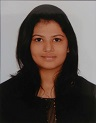
\includegraphics[scale=0.7]{krupa.jpg}\\
 
 \noindent\textbf{{\normalsize  OBJECTIVE}}\\
 \small {Dedicated, energetic and motivated team player seeking an intership position where my potentials will be fully discovered.\\}
 
 \noindent\textbf{{\normalsize  EDUCATION}}\\
 \\
 \begin{tabular}{ |c|c|c|c|c| } 
 	\hline
 	&&&&\\ 
 	\textbf{\large{Examination}} & \textbf{\large{Year of}} & \textbf{\large{Board}} & \textbf{\large{University}} & \textbf{\large{Percentage}} \\
 	& \textbf{Completion} & &  &\textbf{of marks}  \\
 	\hline
 	&&&&\\ 
 	B.E&2020 &R.V. College of & Autonomous  & 9.4\\   
 	(C.S.E)  &  (Pursuing) & Engineering &Affiliated to VTU   &(CGPA: 3 semesters) \\
 	\hline
 	&&&&\\ 
 	XII &2016  & Karnataka State & KMWA P.U.College &  96\% \\
 	&  & & Bengaluru & \\
 	\hline
 	&&&&\\ 
 	X & 2014   & I.C.S.E & Presidency School, & 97.5\% \\
 	&  & & Bengaluru & \\
 	\hline
 \end{tabular}

\vspace{5ex}

\noindent\textbf{{\normalsize PROJECTS}} \begin{enumerate}
	\item 
	\small {\textbf{Planter Bot (December 2017 to March 2018- EYRC-2017,IIT Bombay)}\\\\
		\textbf{Project Objective}\\
		The planter bot traverses different zones in the given arena with the help of image processing techniques
		and depending on the number and type of seedlings detected in each zone, corresponding images are overlayed on the background image.\\
		\textbf{Role and Responsibilities}\\
		Contributed to the algorithm and code of the project\\
		Challenges :Shadow and Glare Removal, Path and Zone Detection , Different image processing techniques for following black and white paths, Image Overlay
		
		\item \textbf{Continuous Care Systems}
		(On-going project in CSE,RVCE in collaboration with Hewlett Packard Enterprise(HPE))\\\\
		\textbf{Project Objective}\\
		Abrupt changes in body conditions and health inspires the need for continuous monitoring and analysis of the human body,especially for patients with long-time illnesses.\\
		Therefore,a coordinated,responsive system with patients and doctors that serves without delay would significantly improve healthcare and enable patients to lead a normal life.\\
		\textbf{Role and Responsibilities}\\
		Ideation of styling the UI for easier recognition of the current condition of the patient being monitored(Dynamic data updation,Regular report generation on the patient side application)\\
		Challenges :Continuous updation of real time data, Getting appropriate sensors for various types of monitoring
	}
	
\end{enumerate}

\vspace{2ex}

\noindent\textbf{{\normalsize  TRAINING AND INTERNSHIP}} \begin{itemize}
	\small {\item 	Completed \textbf{NPTEL} Online Certification on Introduction to Modern Application Development, \textbf{IIT Madras}
		\item	Completed Arduino training conducted by Astra Robotics,RVCE
	}
\end{itemize}
\vspace{2ex}
\noindent\textbf{{\normalsize  TECHNICAL SKILLS}} 

\begin{enumerate}
	\small {\item Programming language : C, Java,Python
		\item Microsoft Office
		\item Boards :  Arduino, Raspberry pi
	}
\end{enumerate}

\vspace{2ex}
\noindent\textbf{{\normalsize SOFT SKILLS}} 

\begin{enumerate}
	\small {\item Good verbal skills, Self-motivation, Adaptability,Time Management, Positive outlook
		\item Attended workshop on Communication skills and professional ethics - Personality development program conducted by \textbf{Genesis Training} (6 days)
	}
\end{enumerate}

\vspace{2ex}
\noindent\textbf{{\normalsize  EXTRA-CURRICULAR ACTIVITIES}} 

\begin{itemize}
	\small {\item Former member of \textbf{Project Garuda},RVCE-India's First Super-mileage Team.
		\item Current member of \textbf{Frequency Club},RVCE.
		\item Currently working on a project(Continuous Care Systems) under \textbf{Hewlett-Packard Enterprise}
		\item Worked on college level projects:Large scale \textbf{image compression} using parallelized LU decomposition, Java (javafx,jdbc,jsp; Database : MySQL),\\}
\end{itemize}

\noindent\textbf{{\normalsize  CO-CURRICULAR ACTIVITIES}} 

\begin{enumerate}
	\small {\item Completed the carnatic vocal junior examination conducted by \textbf{Karnataka Secondary Education Examination Board (KSEEB)}.(Scored first class)
		\item An \textbf{NCC cadet} for 3 years. Attended various march-pasts including the \textbf{Republic Day parade} in Manekshaw Parade Ground,Bangalore.
		\item 	\textbf{National Service Scheme(NSS)} Volunteer
		\item	A member of the \textbf{Entrepreneurship-cell,RVCE}-Been a Master of Ceremonies for various events and have been an active member in the Production and Design team of E-Cell.
		\item Part of the \textbf{rotaract} club of RVCE 
		\item  Painting and art enthusiast(Won several school and college level certificates)
	}
\end{enumerate}

\begin{flushleft}	
	\vspace{2ex}
	\textbf{{\normalsize  Personal Details\\}}
	\vspace{2ex}
	
	\begin{tabular}{l l}
		Name			:  & Krupa Sindhu S\\
		Father’s Name   :  &Srinivas A N\\ 
		Mother’s Name   :  &Roopa Srinivas\\
		Date of Birth	:  &9th June 1998\\
		Gender			:  &Female\\
		Nationality		:  &Indian\\
		Marital Status 	:  &Single\\
		Languages Known	:  &English, Kannada, Hindi\\
		Current location:  &Bangalore\\
	\end{tabular}

\vspace{2ex}
\textbf{{\large Declaration\\}}
\vspace{2ex}
I hereby declare that all the above mentioned information given by me is true and correct to the best of my knowledge.\\
\end{flushleft}
\end{document}
